\chapter{Performance Evaluation}
\label{Performance Evaluation}
\minitoc

Although non-uniform distributed random numbers may be needed in some applications,
for example the user request generator with non-uniform distributed arrival rate in a queuing
system, it is still a majority to have a random sequence with uniform distribution over certain
domain S (this kind of random number generator is called uniform random number generator). 
In order to test the uniformity of a sequence, several methods can be applied.

\section{Balance of Probability}


If a bit sequence is concerned, the uniformity can be justified by comparing the
number of 0's and 1's appeared. That can be accounted with the balance of probability [19],
which defined as$\frac{p-q}{n}$, where $p$ and $q$ are the occurrence frequencies of ``1`` and ``0``,
respectively and $n$ is the number of bits. Figure~\ref{Balance of Probability for old CI} and Figure~\ref{Balance of Probability for new CI} show the balance of probability for a bit
sequence generated by chaotic iterations, showing that the chances to have ``0`` and ``1`` are more or less
the same.
\begin{figure}
\centering
\subfigure[Old CI(Logistic, Logistic)]{\includegraphics[scale=0.34]{images/balance_oldci_ll.eps}
} \hspace{0.5cm}
\subfigure[Old CI(XORshift, XORshift)]{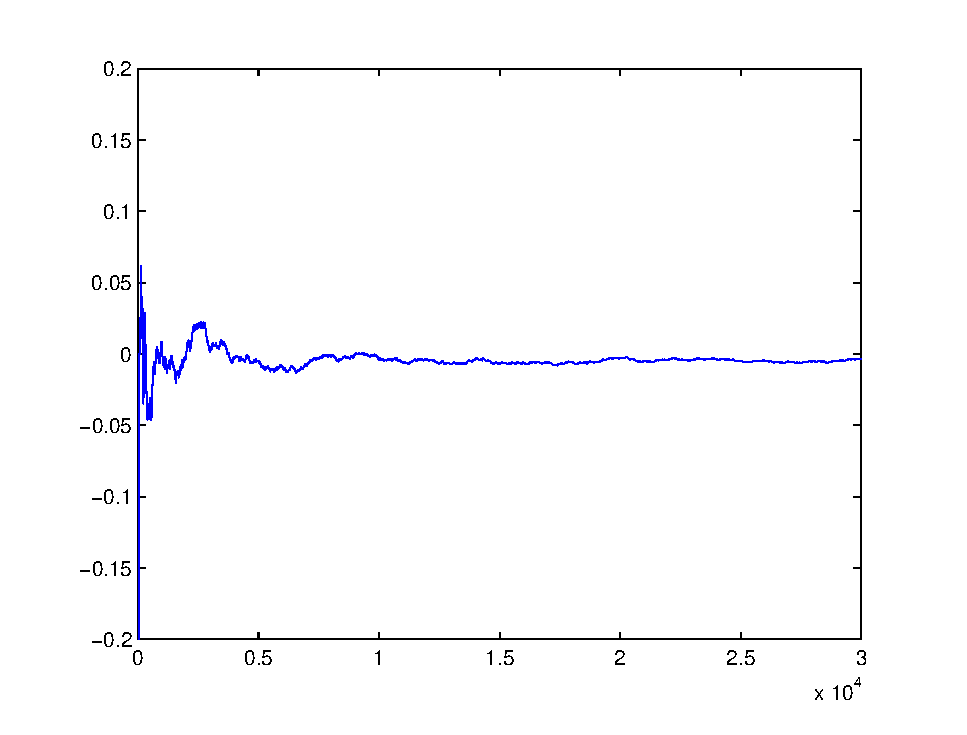
\includegraphics[scale=0.34]{images/balance_oldci_xx.eps}
} \hspace{0.5cm}
\subfigure[Old CI(ISAAC, XORshift)]{\includegraphics[scale=0.34]{images/balance_oldci_xi.eps}
} \hspace{0.5cm}
\subfigure[Old CI(ISAAC, ISAAC)]{\includegraphics[scale=0.34]{images/balance_oldci_ii.eps}
} \hspace{0.5cm}
\caption{Balance of Probability for old CI}
\label{Balance of Probability for old CI}
\end{figure}

\begin{figure}
\centering
\subfigure[New CI(XORshift, XORshift)]{\includegraphics[scale=0.34]{images/balance_newci_xx.eps}
} \hspace{0.5cm}
\subfigure[New CI(ISAAC, XORshift)]{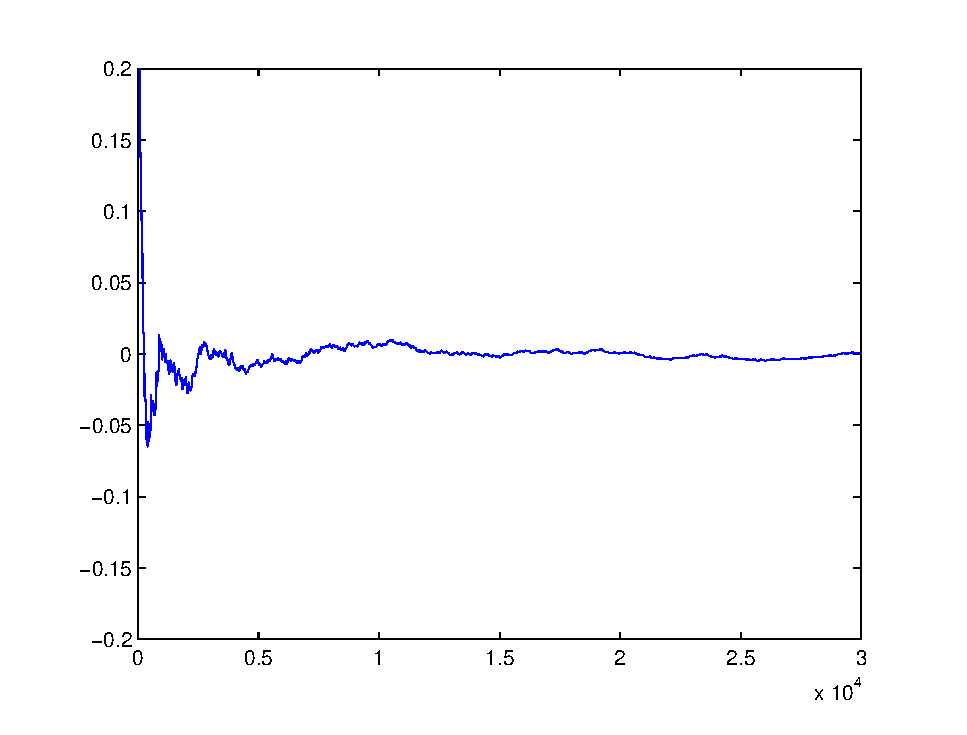
\includegraphics[scale=0.34]{images/balance_newci_xi.eps}
} \hspace{0.5cm}
\subfigure[New CI(ISAAC, ISAAC)]{\includegraphics[scale=0.34]{images/balance_newci_ii.eps}
} \hspace{0.5cm}
\caption{Balance of Probability for new CI}
\label{Balance of Probability for new CI}
\end{figure}

\section{Sensitivity}

As a consequence of its chaotic property, this PRNG is highly sensitive to the initial conditions. To illustrate this property, several initial values are put into the chaotic system. Let $H$ be the number 
of differences between the sequences obtained in this way. Suppose $n$ is the length of these 
sequences. Then the variance ratio $P$, defined by $P = H / n$, is computed. The results are 
shown in Figure~\ref{Sensitivity for old CI} and Figure~\ref{Sensitivity for new CI} ($x$ axis is sequence lengths, $y$ axis is variance ratio $P$). For the two PRNGs, variance 
ratios approach $0.50$, which indicate that the systems are extremely sensitive to the initial 
conditions.
\begin{figure}
\centering
\subfigure[Old CI(Logistic, Logistic)]{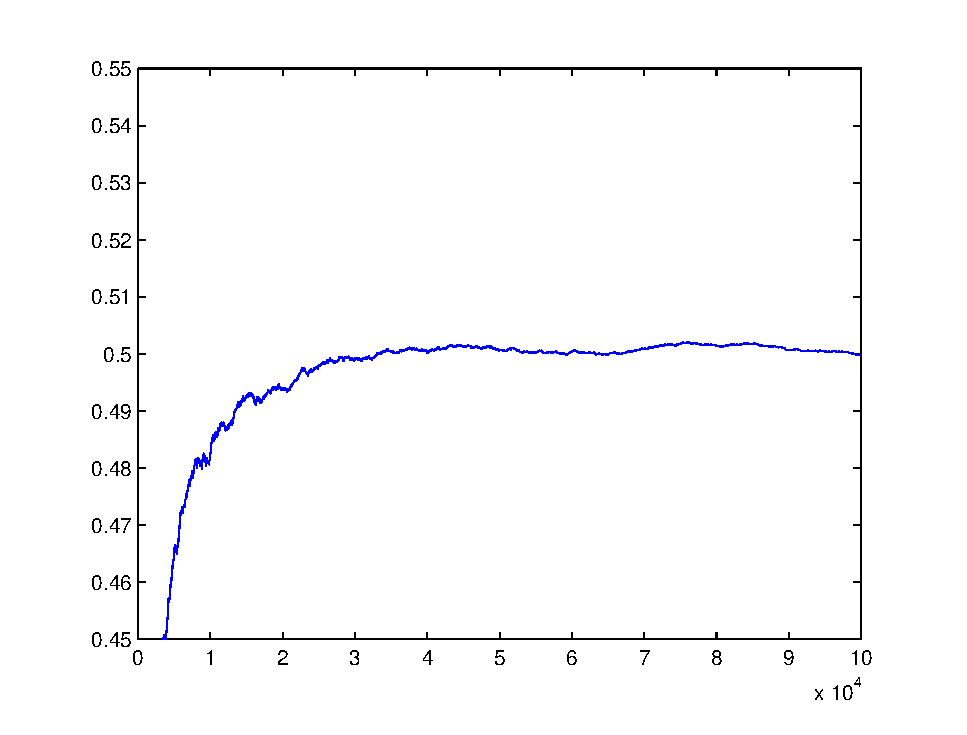
\includegraphics[scale=0.34]{images/Sensitivity_oldci_ll.eps}
} \hspace{0.5cm}
\subfigure[Old CI(XORshift, XORshift)]{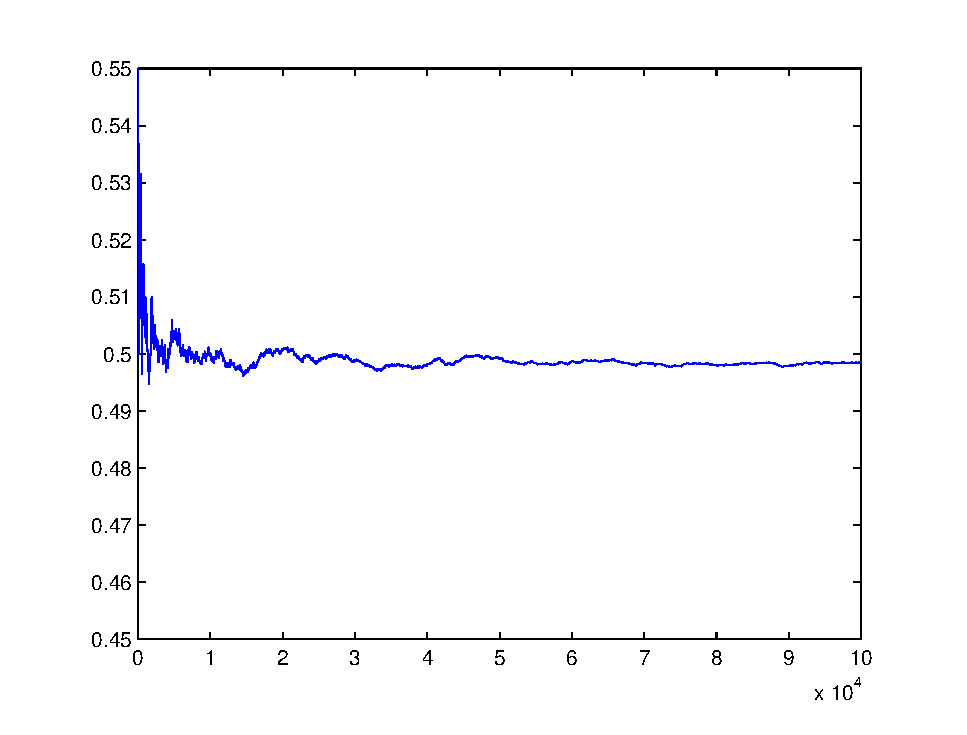
\includegraphics[scale=0.34]{images/Sensitivity_oldci_xx.eps}
} \hspace{0.5cm}
\subfigure[Old CI(ISAAC, XORshift)]{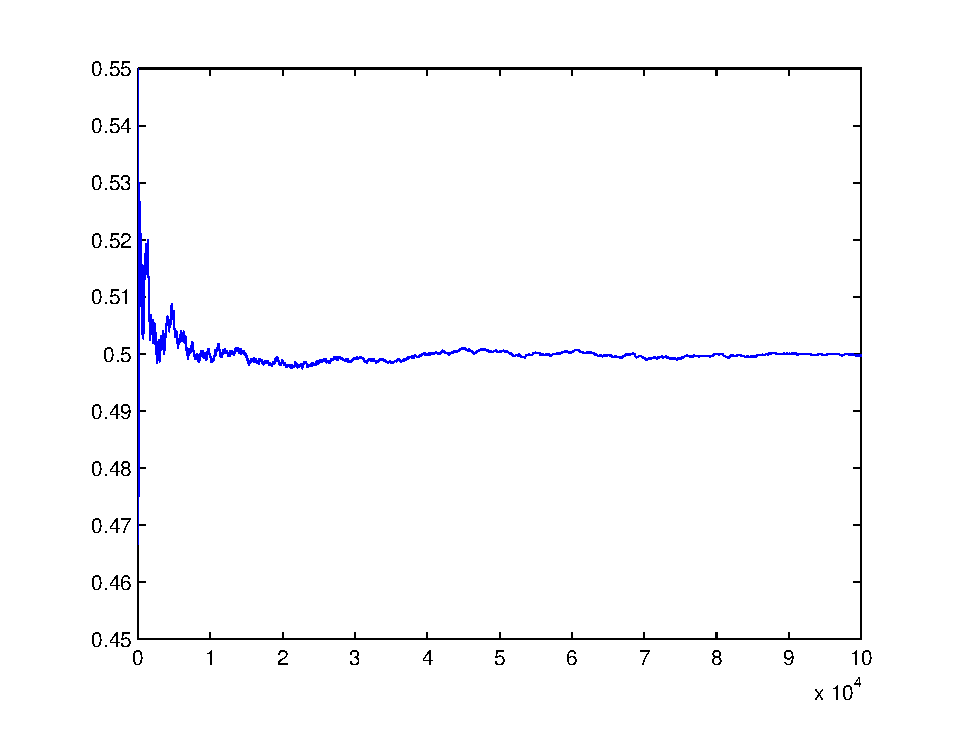
\includegraphics[scale=0.34]{images/Sensitivity_oldci_xi.eps}
} \hspace{0.5cm}
\subfigure[Old CI(ISAAC, ISAAC)]{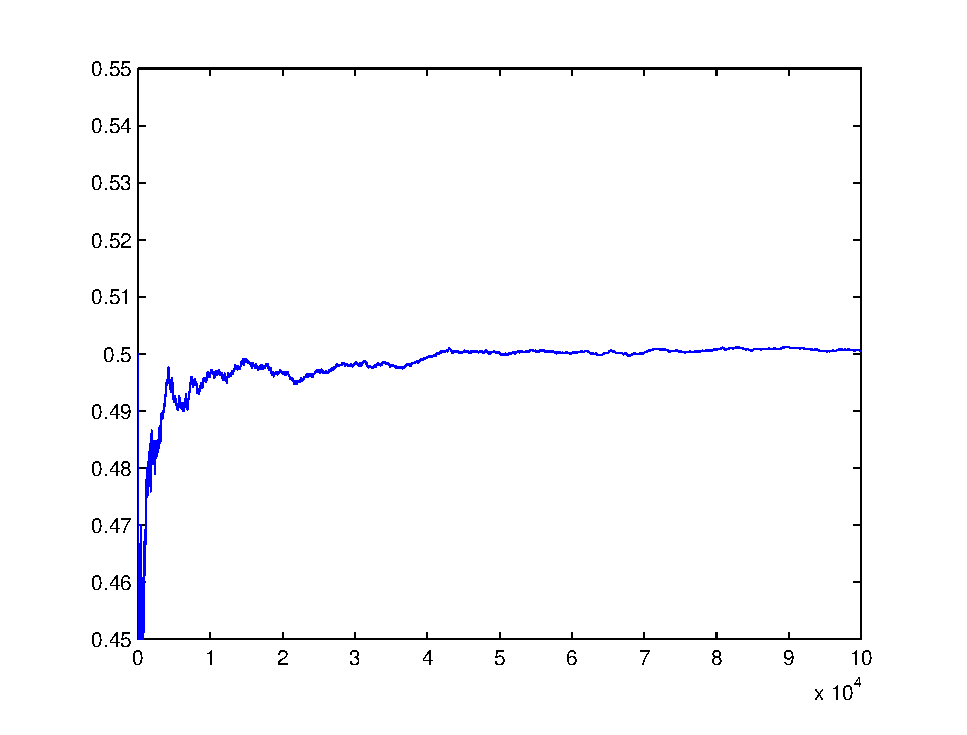
\includegraphics[scale=0.34]{images/Sensitivity_oldci_ii.eps}
} \hspace{0.5cm}
\caption{Sensitivity for old CI}
\label{Sensitivity for old CI}
\end{figure}

\begin{figure}
\centering
\subfigure[New CI(XORshift, XORshift)]{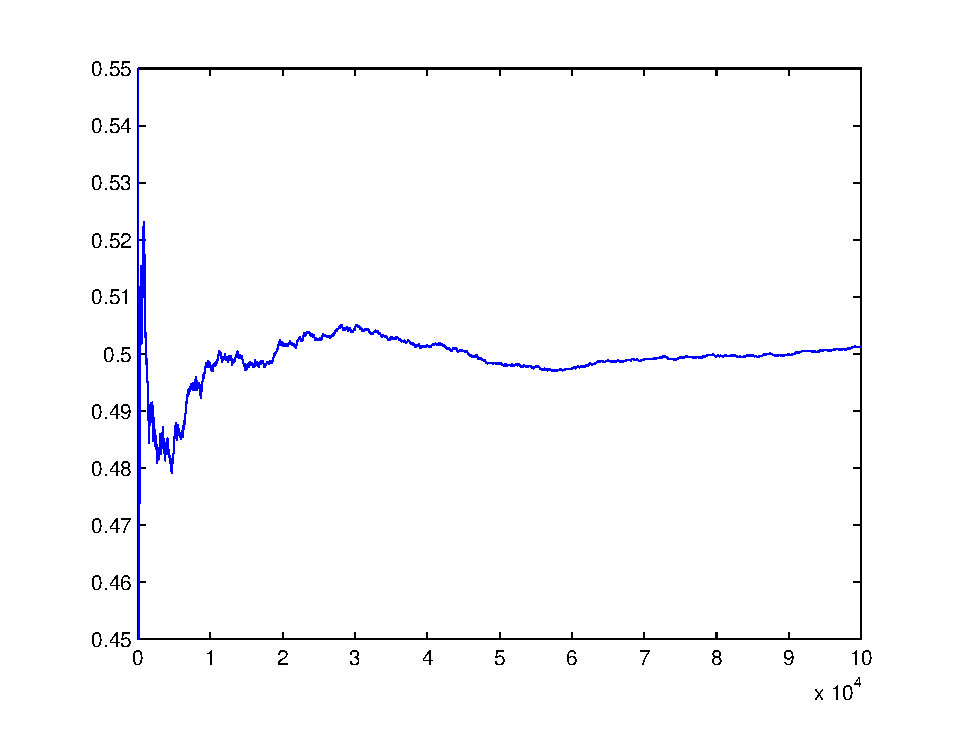
\includegraphics[scale=0.34]{images/Sensitivity_newci_xx.eps}
} \hspace{0.5cm}
\subfigure[New CI(ISAAC, XORshift)]{\includegraphics[scale=0.34]{images/Sensitivity_newci_xi.eps}
} \hspace{0.5cm}
\subfigure[New CI(ISAAC, ISAAC)]{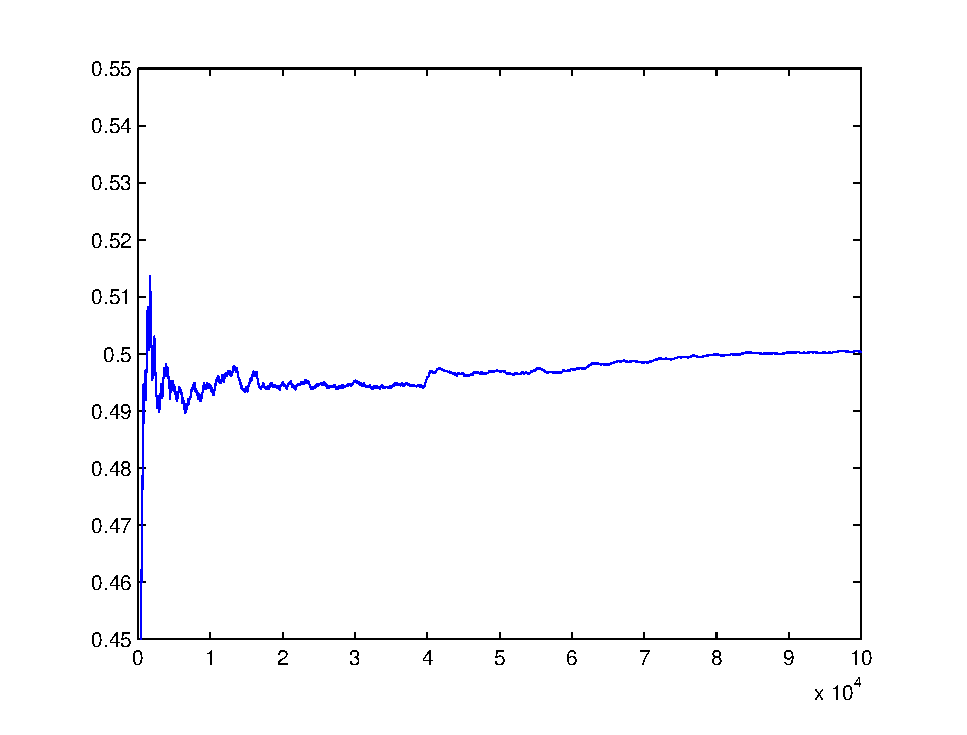
\includegraphics[scale=0.34]{images/Sensitivity_newci_ii.eps}
} \hspace{0.5cm}
\caption{Sensitivity for new CI}
\label{Sensitivity for new CI}
\end{figure}


\section{Pattern}
If a sequence consists of periodic features or repetitive patterns, it is not random [58]. These data patterns existed in the sequence can be revealed by the use of recurrence plot [59], which can be constructed as follows.

Considering a sequence ${x_0,x_1\ldots x_n}$, a vector $y_i$ of dimension $m\geqslant2$ and delay $d\geqslant1$ can be constructed by:
\begin{equation}
\centering
y_i=(x_i,x_{i+d},x_{i+2d},\ldots,x_{i+(m-1)d})
\end{equation}
The recurrence plot is then obtained by plotting a point if the following condition is satisfied:
\begin{equation}
\centering
||y_j-y_i||<t
\end{equation}
where t is a threshold distance.

Figure~\ref{The corresponding recurrence plot for old CI} and Figure~\ref{The corresponding recurrence plot for new CI} depict some sampled  recurrence plots with $m=2$, $d=1$, $t=0.05$, respectively. The points are scattered as shown in Figures, patterns can not easily observed as it is non-periodic and random.
\begin{figure}
\centering
\subfigure[Old CI(Logistic, Logistic)]{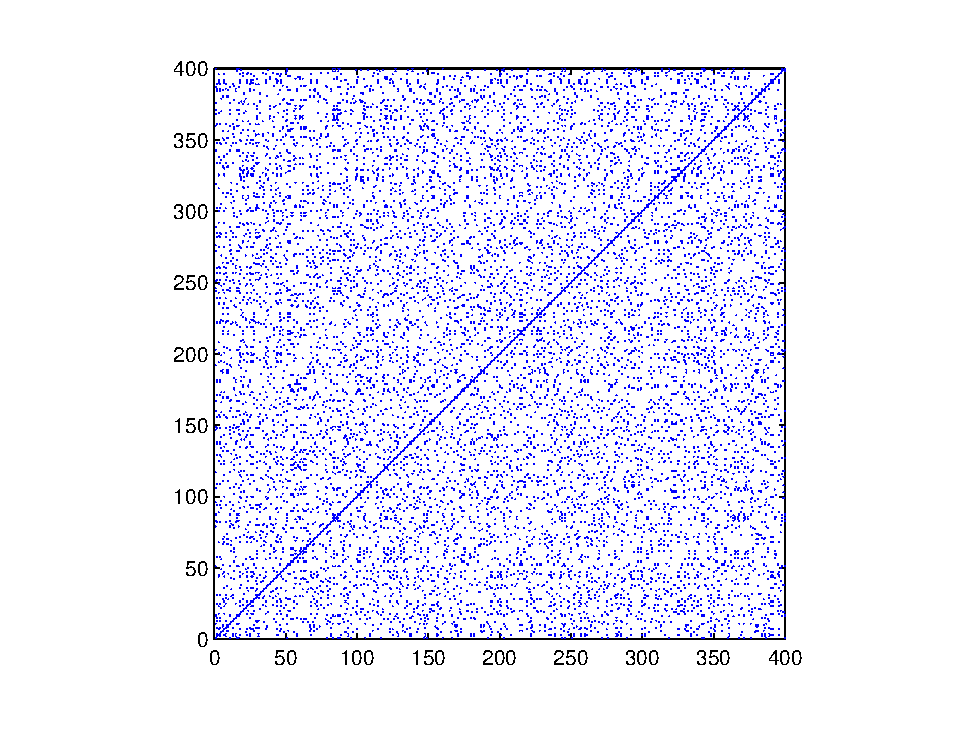
\includegraphics[scale=0.4]{images/pattern_oldci_ll.eps}
} \hspace{0.5cm}
\subfigure[Old CI(XORshift, XORshift)]{\includegraphics[scale=0.4]{images/pattern_oldci_xx.eps}
} \hspace{0.5cm}
\subfigure[Old CI(ISAAC, XORshift)]{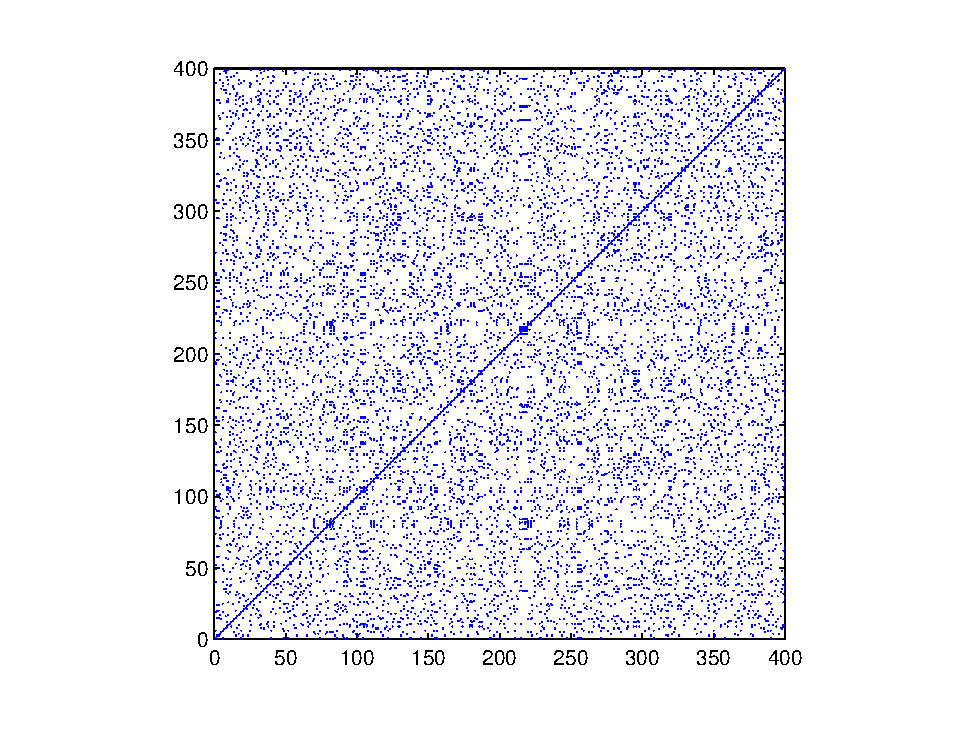
\includegraphics[scale=0.4]{images/pattern_oldci_xi.eps}
} \hspace{0.5cm}
\subfigure[Old CI(ISAAC, ISAAC)]{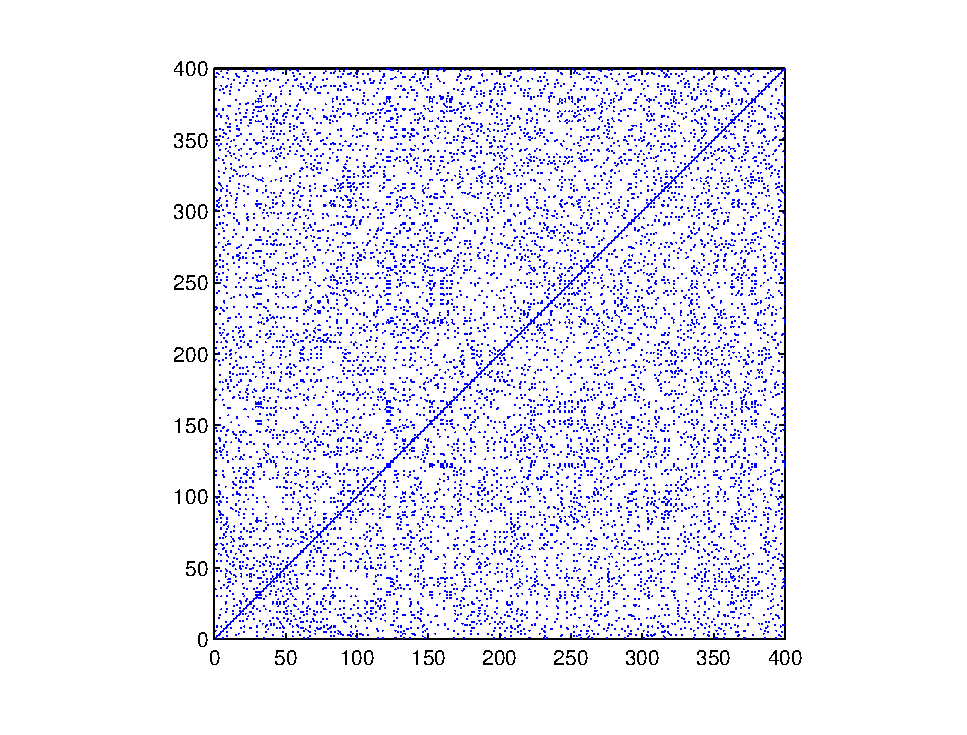
\includegraphics[scale=0.4]{images/pattern_oldci_ii.eps}
} \hspace{0.5cm}
\caption{The corresponding recurrence plot for old CI}
\label{The corresponding recurrence plot for old CI}
\end{figure}

\begin{figure}
\centering
\subfigure[New CI(XORshift, XORshift)]{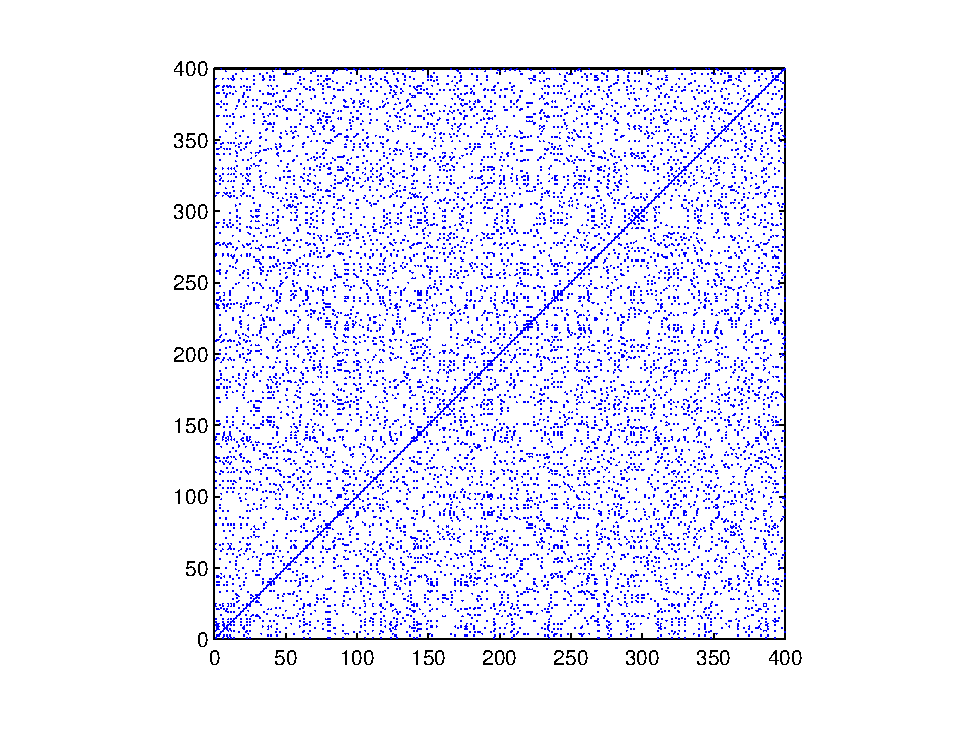
\includegraphics[scale=0.41]{images/pattern_newci_xx.eps}
} \hspace{0.5cm}
\subfigure[New CI(ISAAC, XORshift)]{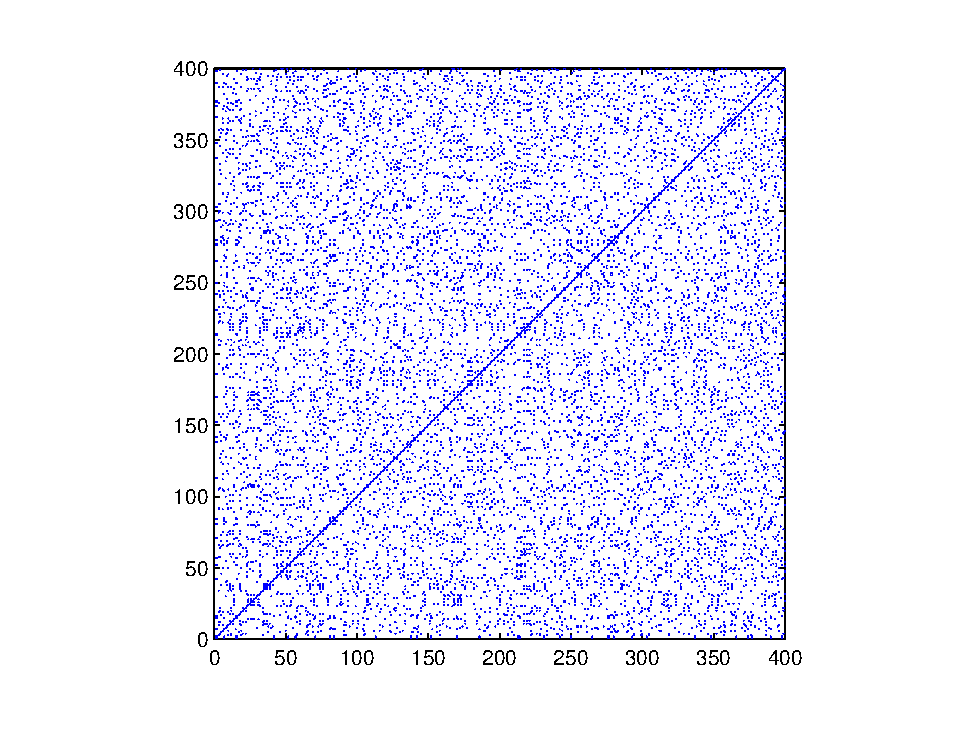
\includegraphics[scale=0.4]{images/pattern_newci_xi.eps}
} \hspace{0.5cm}
\subfigure[New CI(ISAAC, ISAAC)]{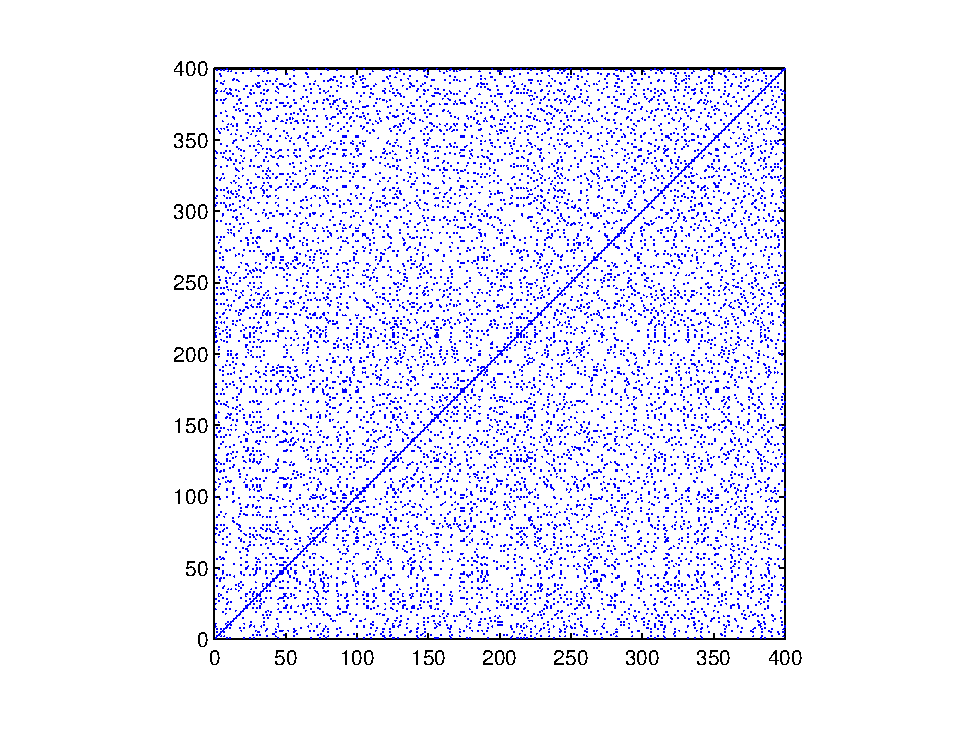
\includegraphics[scale=0.4]{images/pattern_newci_ii.eps}
} \hspace{0.5cm}
\caption{The corresponding recurrence plot for new CI}
\label{The corresponding recurrence plot for new CI}
\end{figure}


\section{Linear complexity}
A sequence is considered to be random only if it cannot be
reconstructed with a short program, or cannot be described by some simple laws. Therefore, if
a sequence is random, it has maximal complexity [60], and data compression is nearly
impossible.

The linear complexity (LC) of a sequence is the size in bits of the shortest linear feedback shift register (LFSR) which can produce this sequence. This value measures the difficulty of generating -- and perhaps analyzing -- a particular sequence.
Indeed, the randomness of a given sequence can be linked to the size of the smallest program that can produce it. LC is the size required by a LFSR to be able to produce the given sequence. The Berlekamp-Massey algorithm can measure this LC, which might be used to evaluate the ``security'' of a pseudo-random sequence.

It can be seen in Figure~\ref{Linear complexity for old CI} and Figure~\ref{Linear complexity for new CI} that the LC curves of sample sequences of 2000 b are close to the ideal line $C_i=i/2$, which imply that the generator has high linear complexity. 
\begin{figure}
\centering
\subfigure[Old CI(Logistic, Logistic)]{\includegraphics[scale=0.34]{images/linear_complexity_oldci_ll.eps}
} \hspace{0.5cm}
\subfigure[Old CI(XORshift, XORshift)]{\includegraphics[scale=0.34]{images/linear_complexity_oldci_xx.eps}
} \hspace{0.5cm}
\subfigure[Old CI(ISAAC, XORshift)]{\includegraphics[scale=0.34]{images/linear_complexity_oldci_xi.eps}
} \hspace{0.5cm}
\subfigure[Old CI(ISAAC, ISAAC)]{\includegraphics[scale=0.34]{images/linear_complexity_oldci_ii.eps}
} \hspace{0.5cm}
\caption{Linear complexity for old CI}
\label{Linear complexity for old CI}
\end{figure}

\begin{figure}
\centering
\subfigure[New CI(XORshift, XORshift)]{\includegraphics[scale=0.34]{images/linear_complexity_newci_xx.eps}
} \hspace{0.5cm}
\subfigure[New CI(ISAAC, XORshift)]{\includegraphics[scale=0.34]{images/linear_complexity_newci_xi.eps}
} \hspace{0.5cm}
\subfigure[New CI(ISAAC, ISAAC)]{\includegraphics[scale=0.34]{images/linear_complexity_newci_ii.eps}
} \hspace{0.5cm}
\caption{Linear complexity for new CI}
\label{Linear complexity for new CI}
\end{figure}


\section{Uniform distribution}

Figure~\ref{Second order distribution for old CI} and Figure~\ref{Second order distribution for new CI} give a 3D graphic representation of the distribution of a random sequence obtained by our generators. The point cloud presents a uniform distribution that tends to fill the complete 3D space, as expected for a random signal. To obtain this cloud, we have first changed the binary sequence to a $N$-bit integer sequence $x_1$, $x_2$, $x_3$, $x_4$... Then we have plot $\left(\frac{x_1}{2^N},\frac{x_2}{2^N},\frac{x_3}{2^N}\right), \left(\frac{x_2}{2^N},\frac{x_3}{2^N},\frac{x_4}{2^N}\right)$...

\begin{figure}
\centering
\subfigure[Old CI(Logistic, Logistic)]{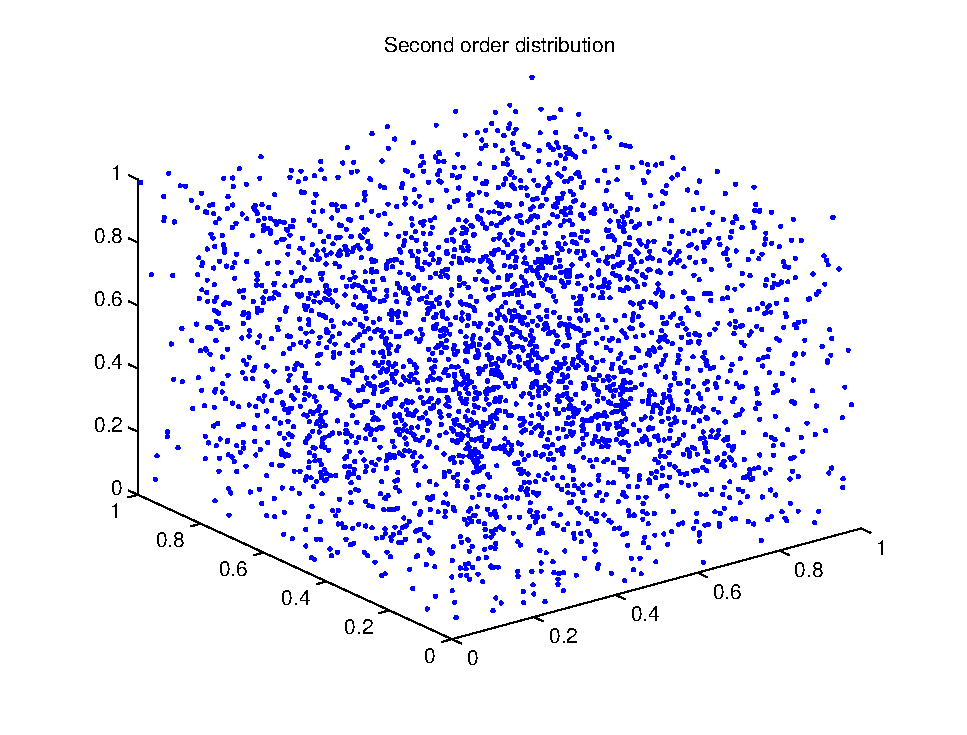
\includegraphics[scale=0.34]{images/distribution_oldci_ll.eps}
} \hspace{0.5cm}
\subfigure[Old CI(XORshift, XORshift)]{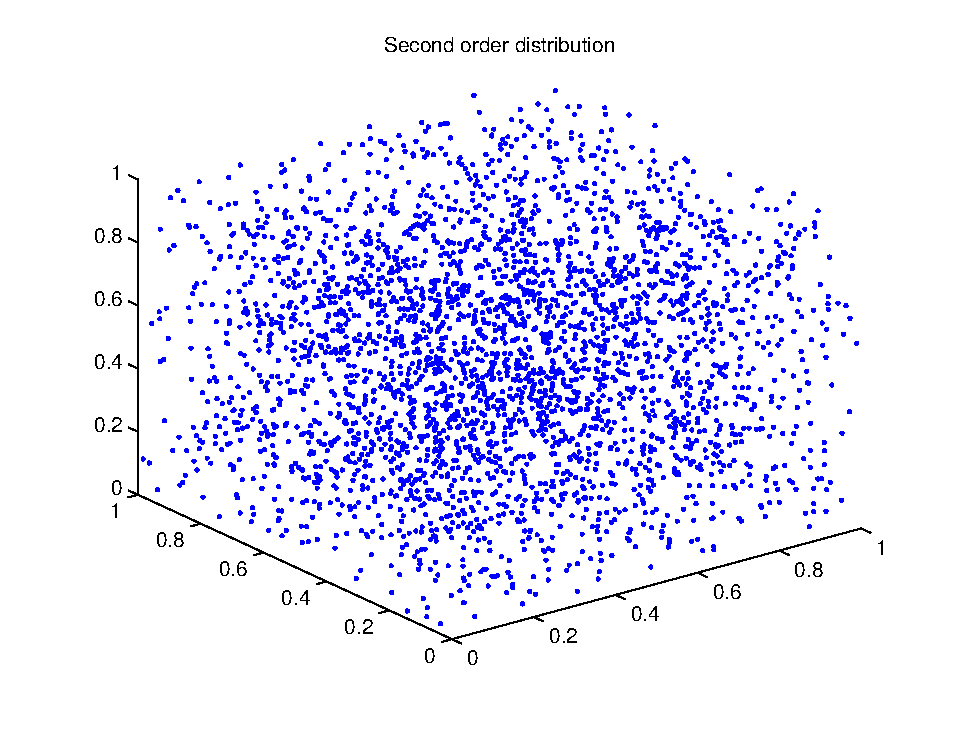
\includegraphics[scale=0.34]{images/distribution_oldci_xx.eps}
\label{Old CI(XORshift, XORshift)}} \hspace{0.5cm}
\subfigure[Old CI(ISAAC, XORshift)]{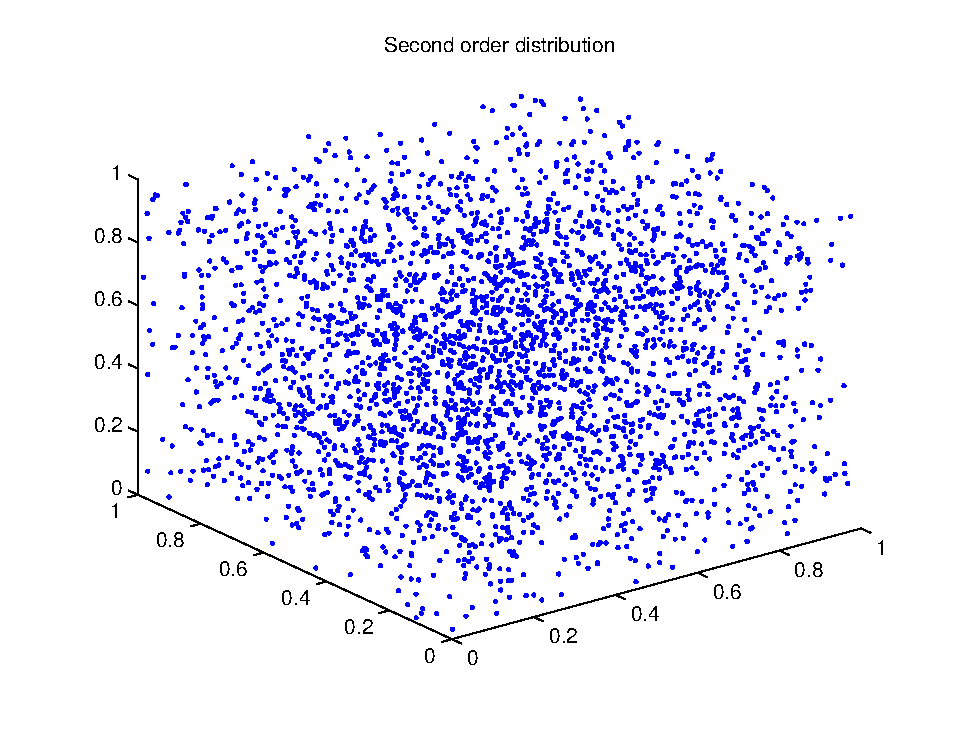
\includegraphics[scale=0.34]{images/distribution_oldci_xi.eps}
\label{Old CI(ISAAC, XORshift)}} \hspace{0.5cm}
\subfigure[Old CI(ISAAC, ISAAC)]{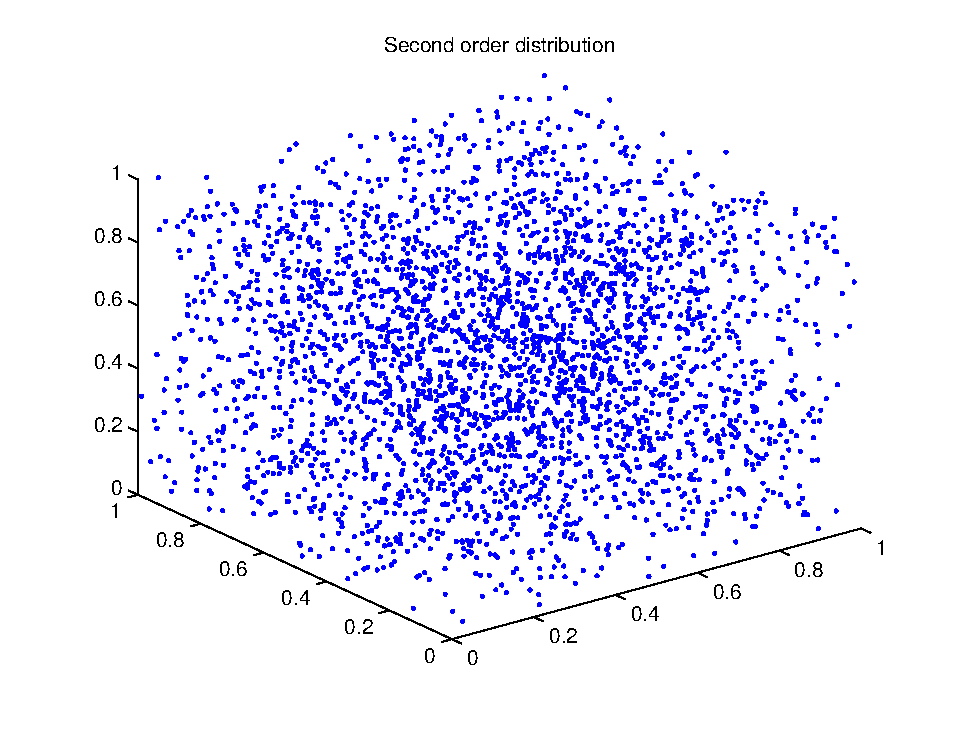
\includegraphics[scale=0.34]{images/distribution_oldci_ii.eps}
\label{Old CI(ISAAC, ISAAC)}} \hspace{0.5cm}
\caption{Second order distribution for old CI}
\label{Second order distribution for old CI}
\end{figure}

\begin{figure}
\centering
\subfigure[New CI(XORshift, XORshift)]{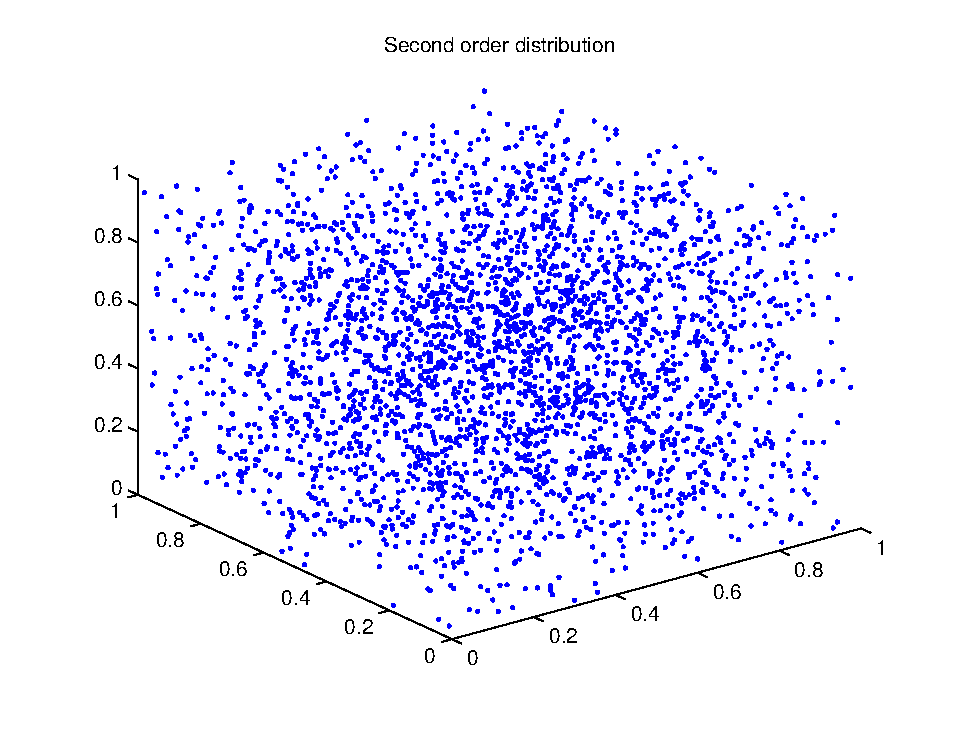
\includegraphics[scale=0.34]{images/distribution_newci_xx.eps}
} \hspace{0.5cm}
\subfigure[New CI(ISAAC, XORshift)]{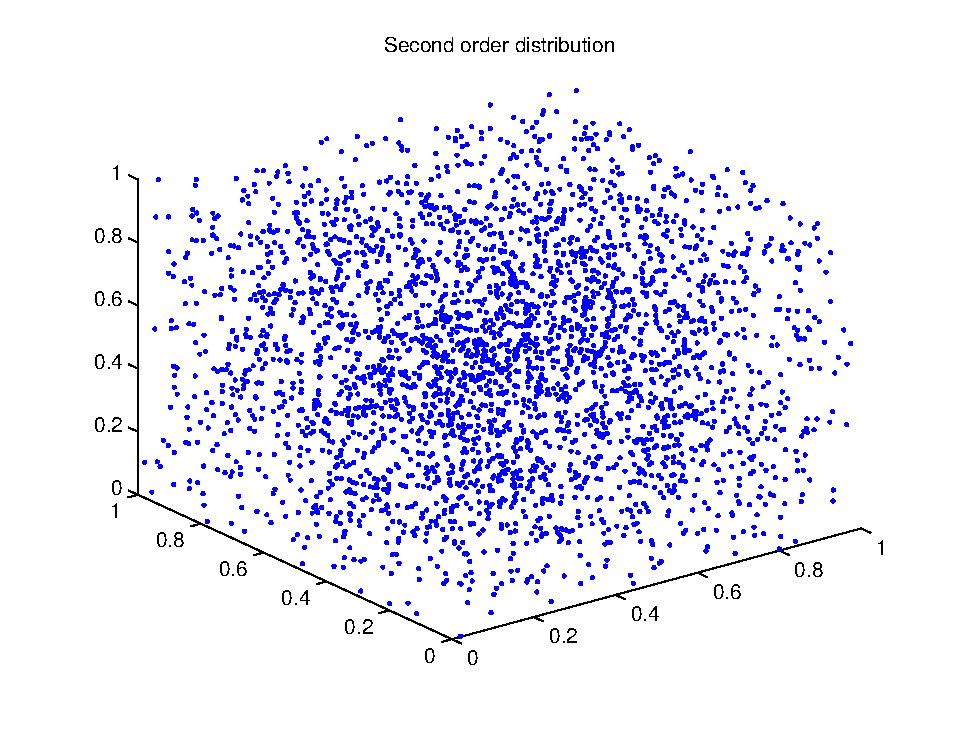
\includegraphics[scale=0.34]{images/distribution_newci_xi.eps}
} \hspace{0.5cm}
\subfigure[New CI(ISAAC, ISAAC)]{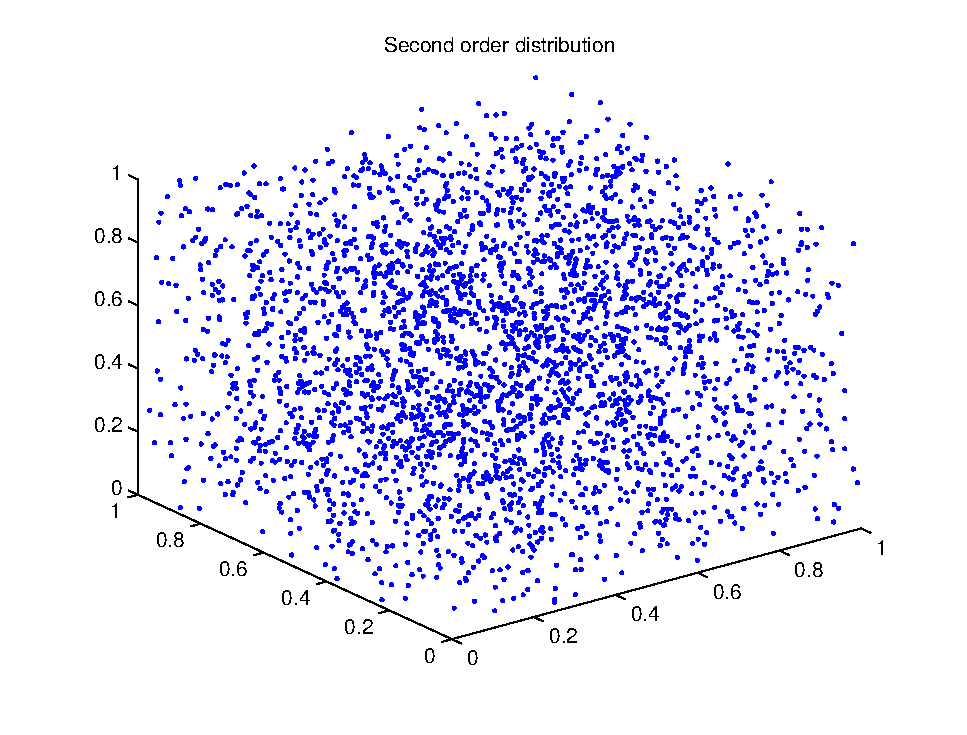
\includegraphics[scale=0.34]{images/distribution_newci_ii.eps}
} \hspace{0.5cm}
\caption{Second order distribution for new CI}
\label{Second order distribution for new CI}
\end{figure}


\section{Auto-correlation and cross-correlation}
Since the number in a random sequence should be unpredictable and hence uncorrelated,
the auto-correlation and the cross-correlation between sequences can also be used to reflect
the randomness of a sequence. These correlation values are also the prime indices when a
random sequence is to be used in spread-spectrum communications [57].

Let $\{u\}$ and $\{v\}$ be two binary $(-1,+1)$-value sequences of length $n$, the aperiodic
auto-correlation function $C_{uu}(l)$ and the aperiodic cross-correlation function $C_{uv}(l)$ are defined
in Equation (\ref{auto}) and (\ref{cross}), respectively.
\begin{equation}
\label{auto}
C_{u,u}(l)=
\left\{
\begin{array}{llc}
\sum_{i=0}^{n-1-l} u_{i}u_{i+l} & \text{ if }&0\leqslant l\leqslant n-1\\
\sum_{i=0}^{n-1+l} u_{i-l}u_{i}  & \text{ if }&1-n\leqslant l\leqslant 0 \\
0 & \text{ if }&|l|\geqslant n\\
\end{array}
\right.
\end{equation}
\begin{equation}
\label{cross}
C_{u,v}(l)=
\left\{
\begin{array}{llc}
\sum_{i=0}^{n-1-l} u_{i}v_{i+l} & \text{ if }&0\leqslant l\leqslant n-1\\
\sum_{i=0}^{n-1+l} u_{i-l}v_{i}  & \text{ if }&1-n\leqslant l\leqslant 0 \\
0 & \text{ if }&|l|\geqslant n\\
\end{array}
\right.
\end{equation}


The auto-correlation and cross-correlation of the symbolic sequences are respectively given in Figure.~\ref{autocorr for old CI}, Figure.~\ref{autocorr for new CI}, Figure.~\ref{intercorr for old CI} and Figure.~\ref{intercorr for new CI}demonstrating a nice nature. It can be seen that this sequences have $\delta$-like auto-correlation which is required for a good PRBNG. The sequences generated with different initial values will have zero cross-correlation due to the sensitive dependence on initial conditions. 



\begin{figure}
\centering
\subfigure[Old CI(Logistic, Logistic)]{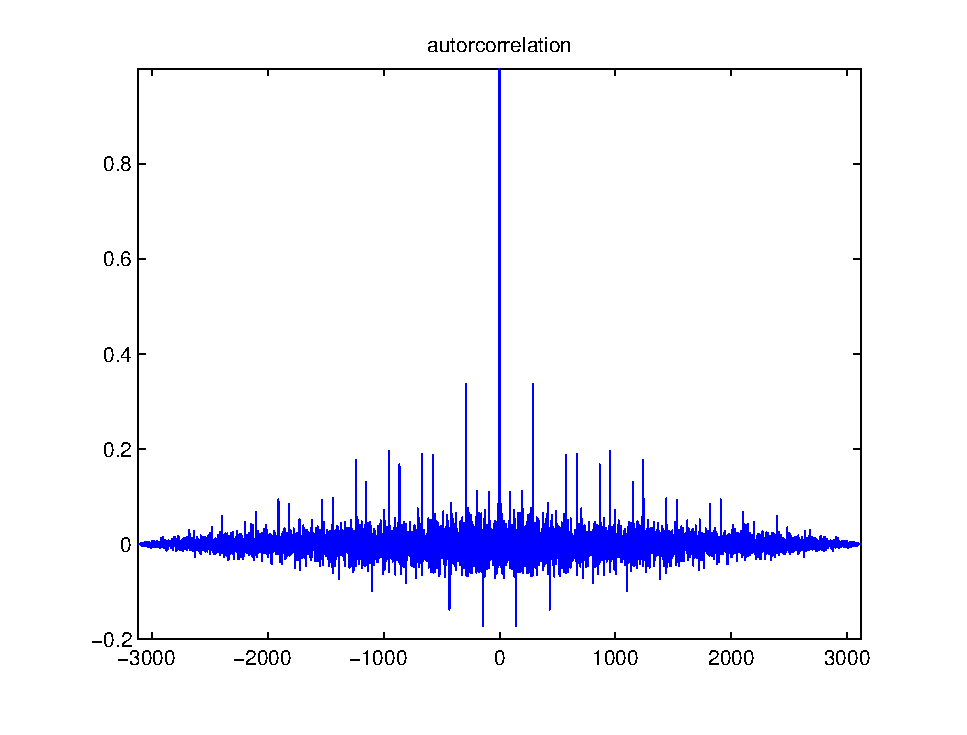
\includegraphics[scale=0.34]{images/autocorr_oldci_ll.eps}
} \hspace{0.5cm}
\subfigure[Old CI(XORshift, XORshift)]{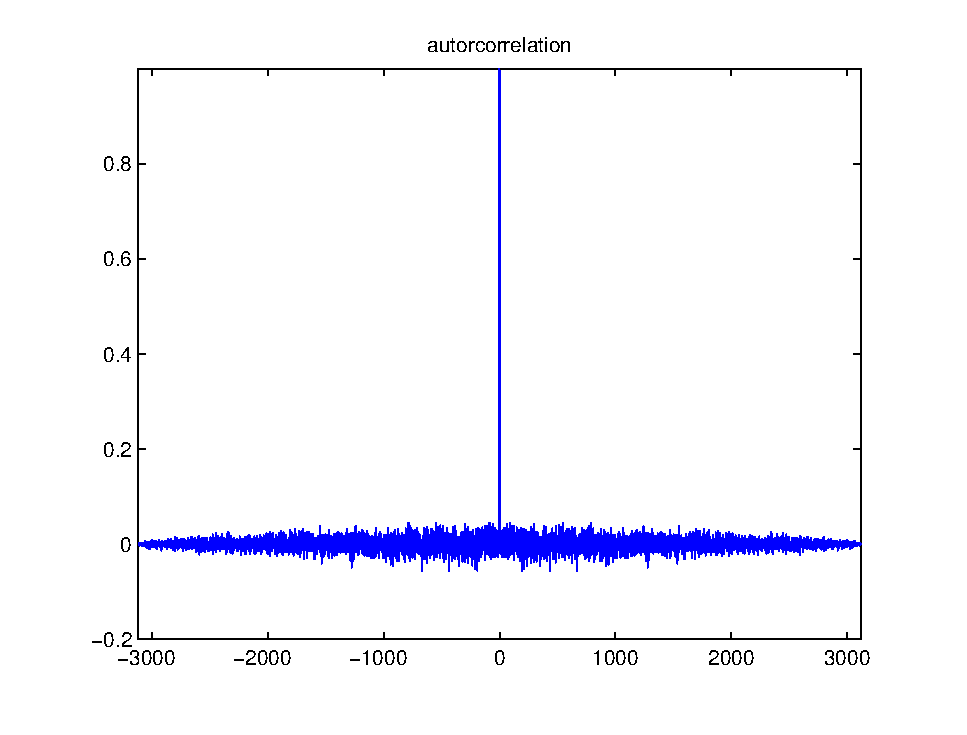
\includegraphics[scale=0.34]{images/autocorr_oldci_xx.eps}
} \hspace{0.5cm}
\subfigure[Old CI(ISAAC, XORshift)]{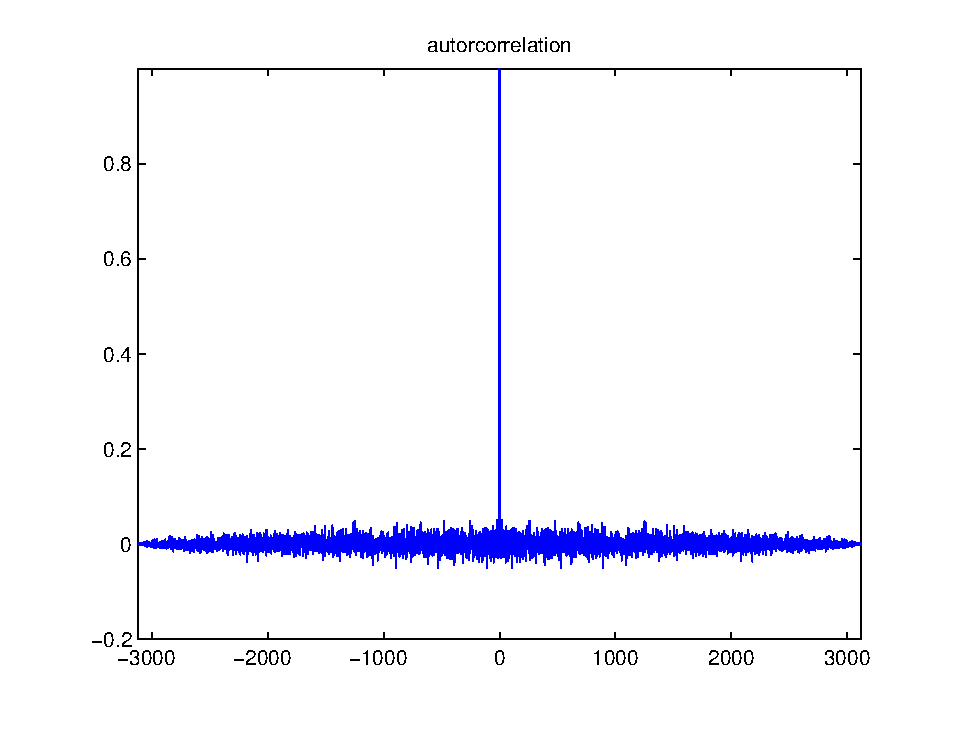
\includegraphics[scale=0.34]{images/autocorr_oldci_xi.eps}
} \hspace{0.5cm}
\subfigure[Old CI(ISAAC, ISAAC)]{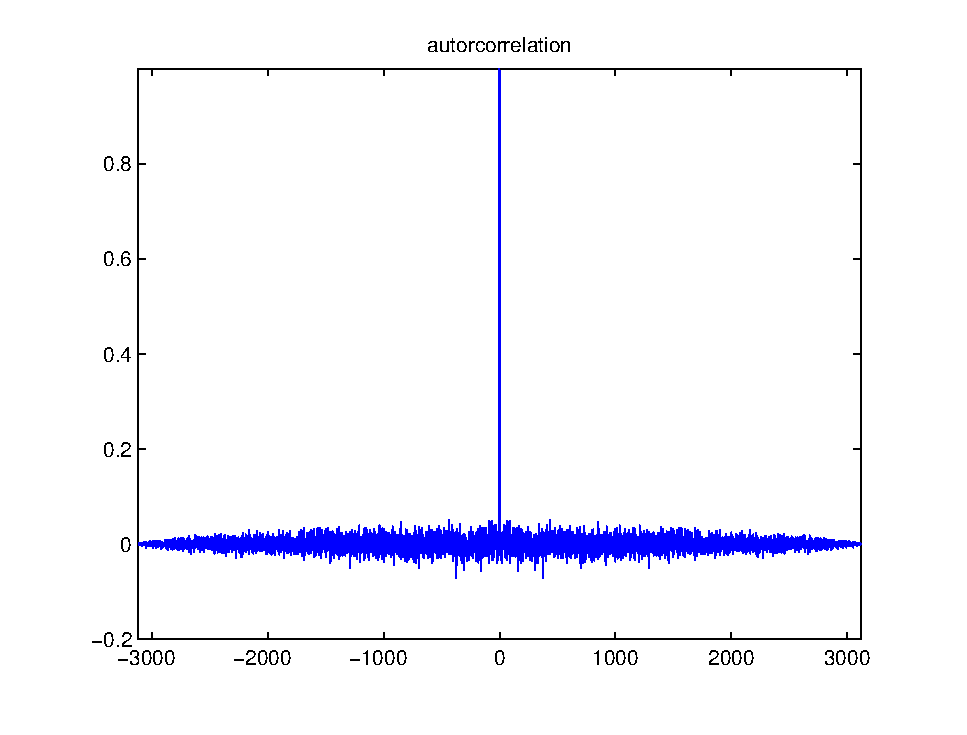
\includegraphics[scale=0.34]{images/autocorr_oldci_ii.eps}
} \hspace{0.5cm}
\caption{Auto-correlation for old CI}
\label{autocorr for old CI}
\end{figure}

\begin{figure}
\centering
\subfigure[New CI(XORshift, XORshift)]{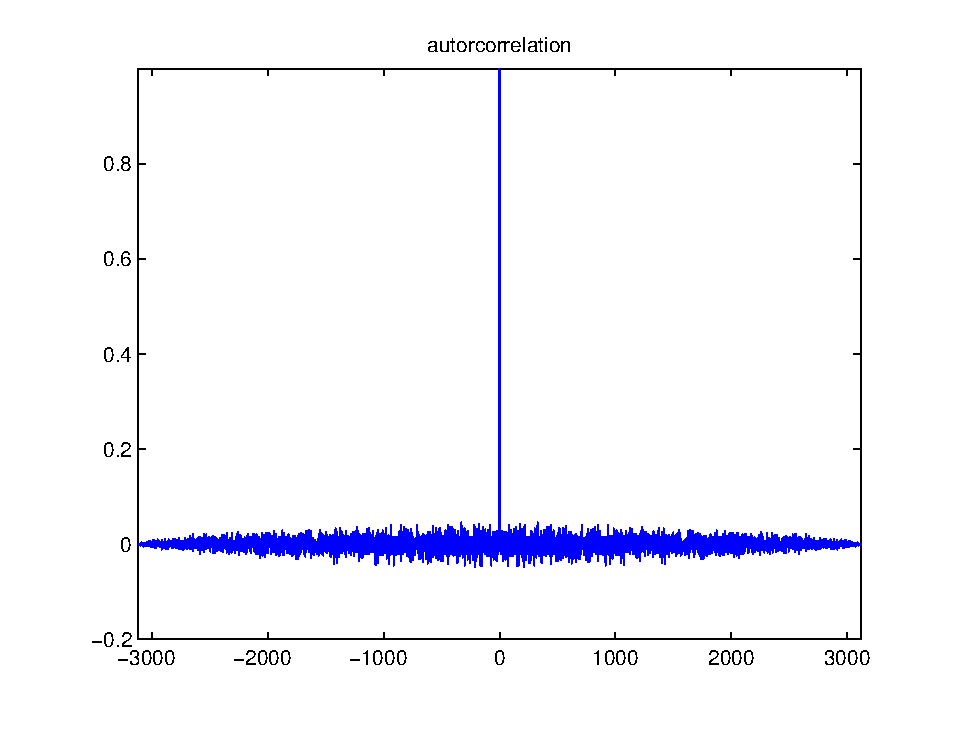
\includegraphics[scale=0.34]{images/autocorr_newci_xx.eps}
} \hspace{0.5cm}
\subfigure[New CI(ISAAC, XORshift)]{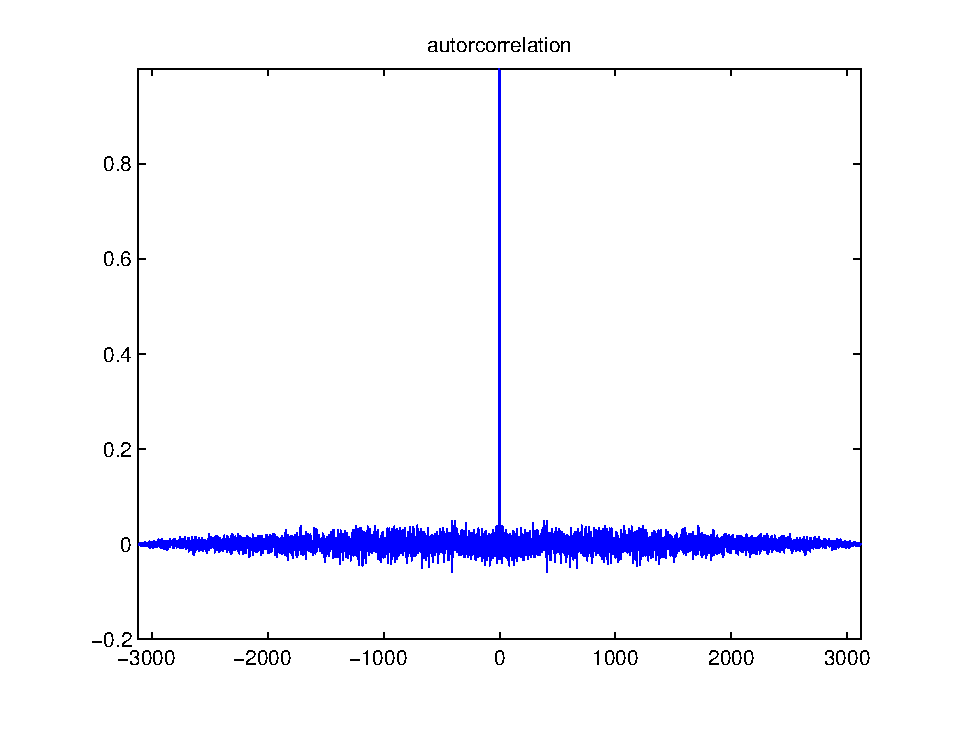
\includegraphics[scale=0.34]{images/autocorr_newci_xi.eps}
} \hspace{0.5cm}
\subfigure[New CI(ISAAC, ISAAC)]{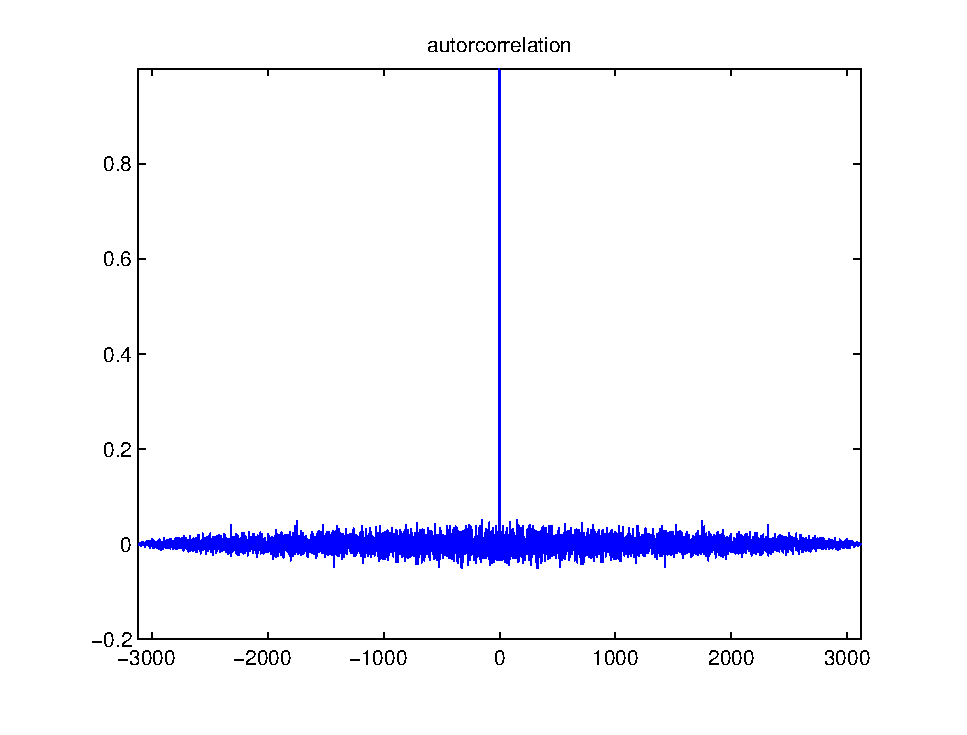
\includegraphics[scale=0.34]{images/autocorr_newci_ii.eps}
} \hspace{0.5cm}
\caption{Auto-correlation for new CI}
\label{autocorr for new CI}
\end{figure}

\begin{figure}
\centering
\subfigure[Old CI(Logistic, Logistic)]{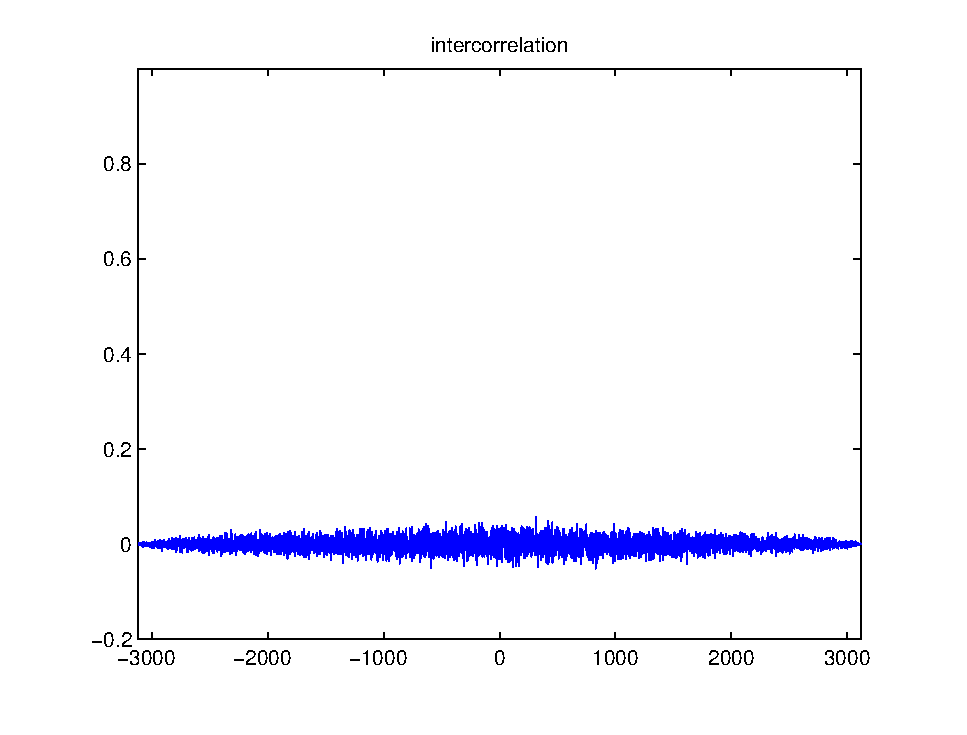
\includegraphics[scale=0.34]{images/intercorr_oldci_ll.eps}
} \hspace{0.5cm}
\subfigure[Old CI(XORshift, XORshift)]{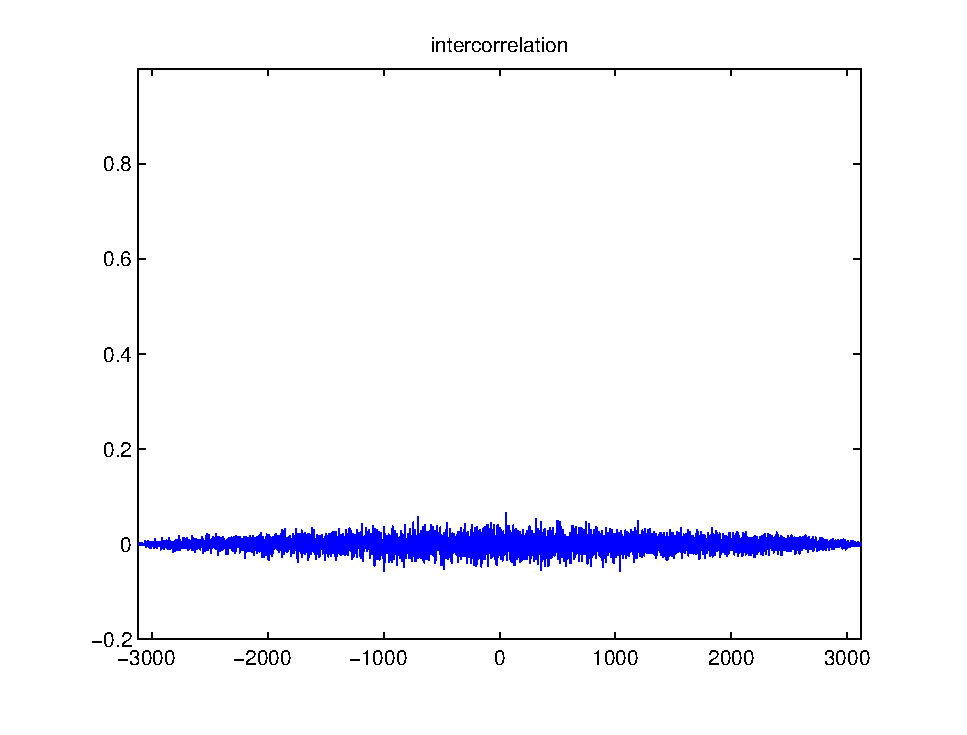
\includegraphics[scale=0.34]{images/intercorr_oldci_xx.eps}
} \hspace{0.5cm}
\subfigure[Old CI(ISAAC, XORshift)]{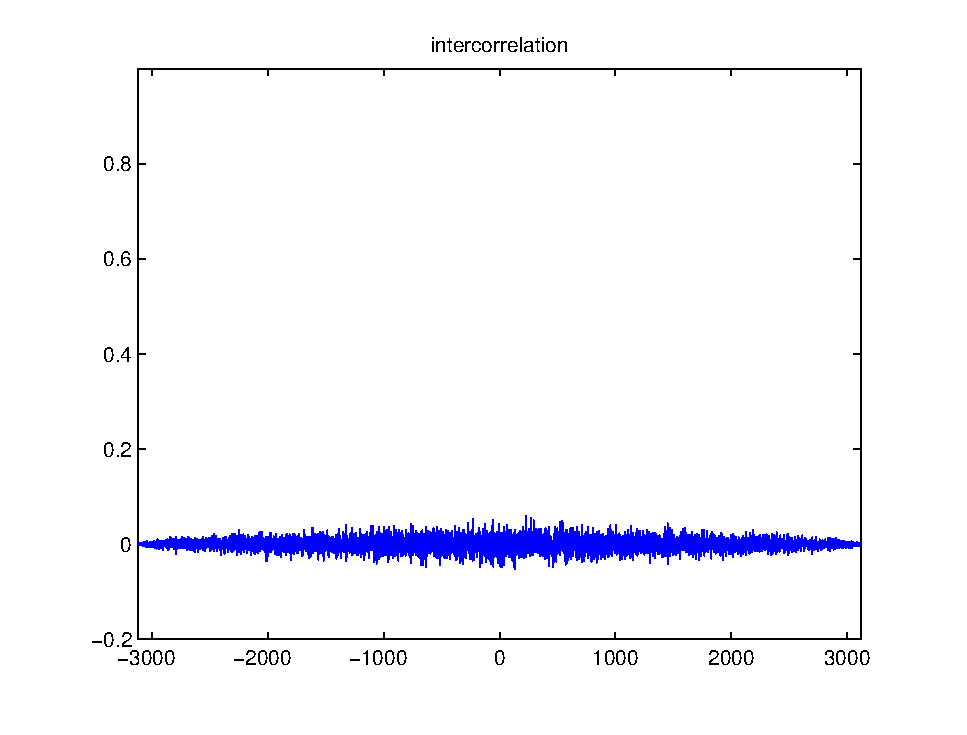
\includegraphics[scale=0.34]{images/intercorr_oldci_xi.eps}
} \hspace{0.5cm}
\subfigure[Old CI(ISAAC, ISAAC)]{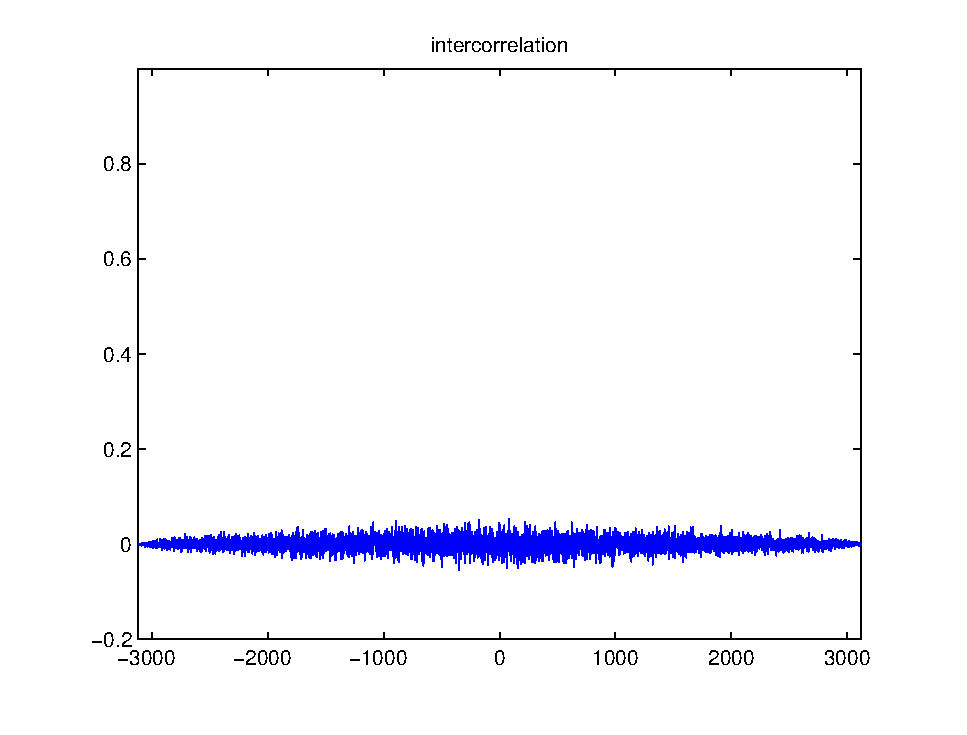
\includegraphics[scale=0.34]{images/intercorr_newci_ii.eps}
} \hspace{0.5cm}
\caption{Cross-correlation for old CI}
\label{intercorr for old CI}
\end{figure}

\begin{figure}
\centering
\subfigure[New CI(XORshift, XORshift)]{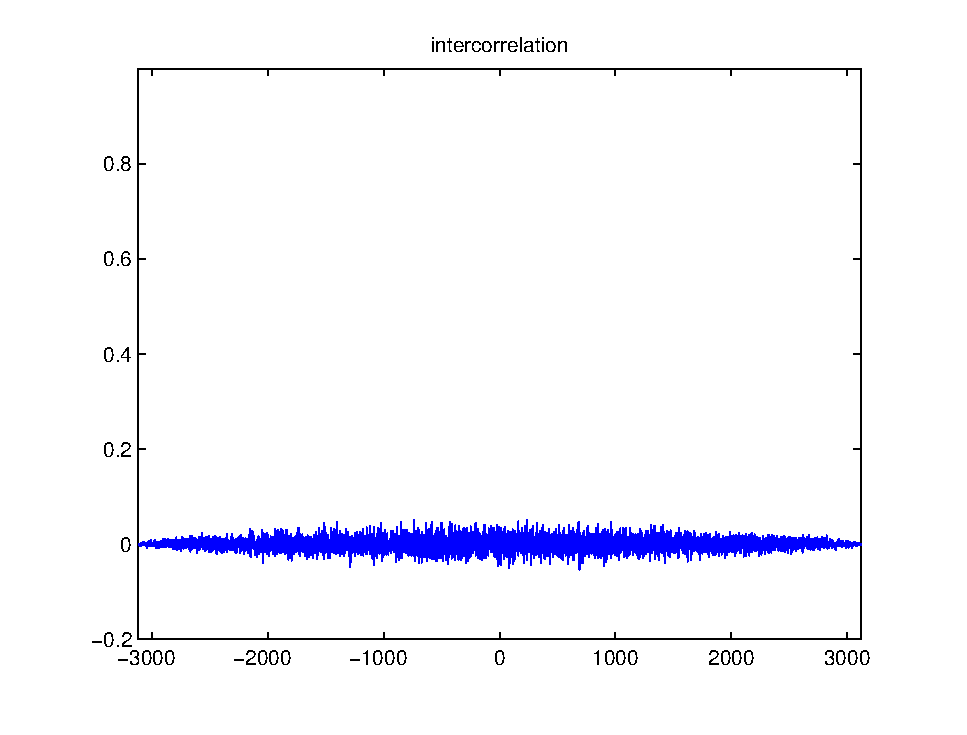
\includegraphics[scale=0.34]{images/intercorr_newci_xx.eps}
} \hspace{0.5cm}
\subfigure[New CI(ISAAC, XORshift)]{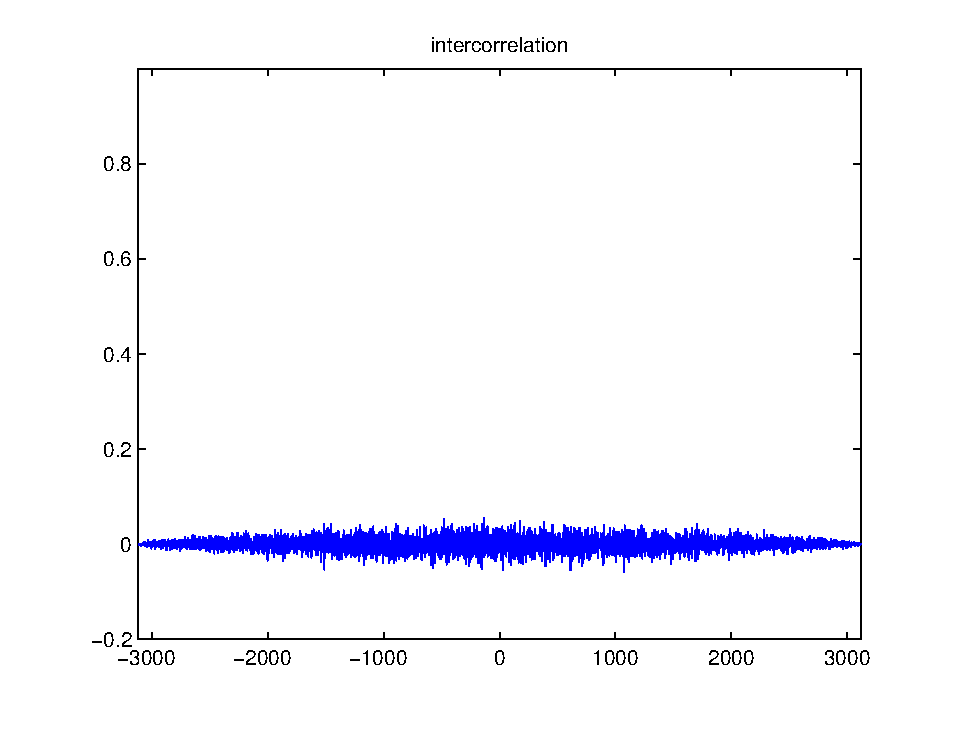
\includegraphics[scale=0.34]{images/intercorr_newci_xi.eps}
} \hspace{0.5cm}
\subfigure[New CI(ISAAC, ISAAC)]{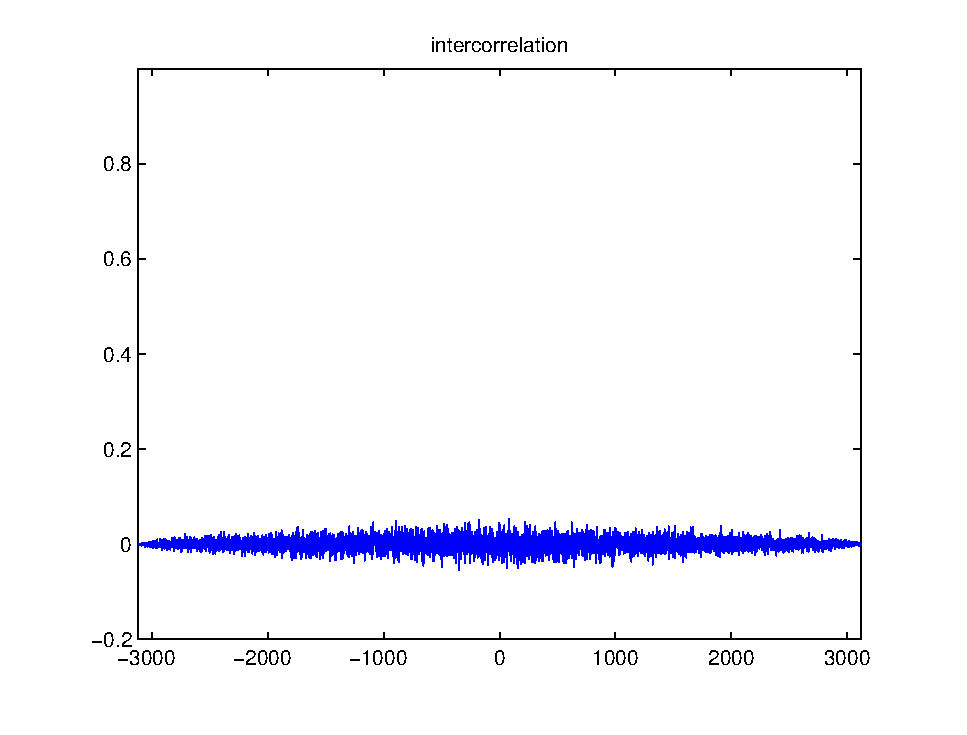
\includegraphics[scale=0.34]{images/intercorr_newci_ii.eps}
} \hspace{0.5cm}
\caption{Cross-correlation for new CI}
\label{intercorr for new CI}
\end{figure}
\section{FFT}

The FFT of the sequences (Figure.~\ref{FFT for old CI} and Figure.~\ref{FFT for new CI}) are performed and the corresponding power spectrums are computed. Some complete flat power spectrums, with almost equal frequency contribution for all frequencies, are indicative of a total random series.

\begin{figure}
\centering
\subfigure[Old CI(Logistic, Logistic)]{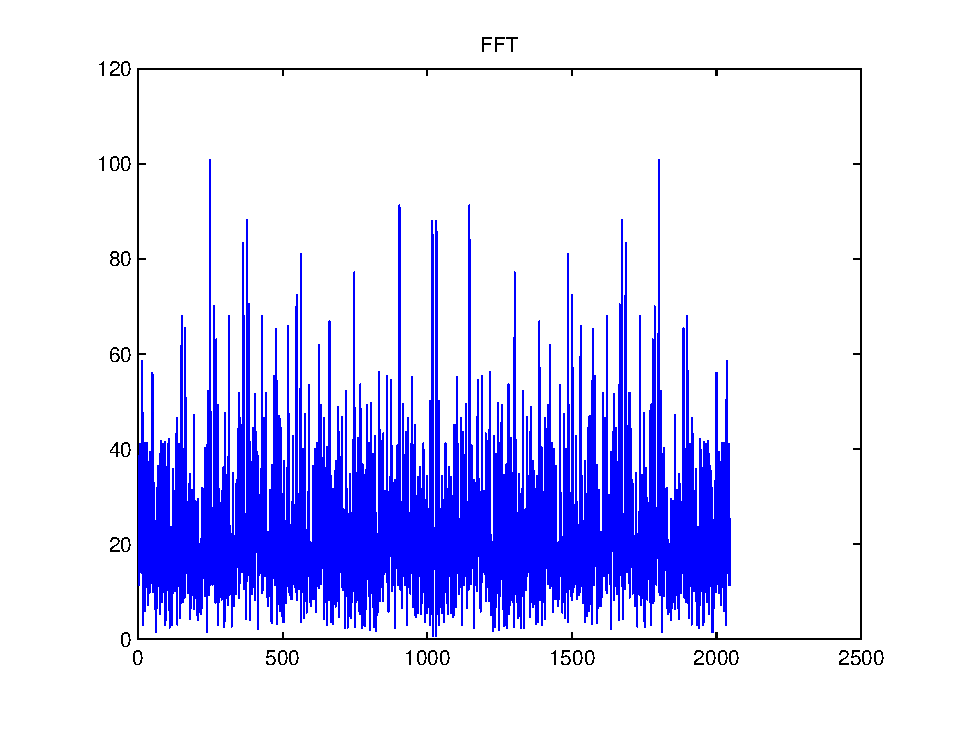
\includegraphics[scale=0.34]{images/fft_oldci_ll.eps}
} \hspace{0.5cm}
\subfigure[Old CI(XORshift, XORshift)]{\includegraphics[scale=0.34]{images/fft_oldci_xx.eps}
} \hspace{0.5cm}
\subfigure[Old CI(ISAAC, XORshift)]{\includegraphics[scale=0.34]{images/fft_oldci_xi.eps}
} \hspace{0.5cm}
\subfigure[Old CI(ISAAC, ISAAC)]{\includegraphics[scale=0.34]{images/fft_oldci_ii.eps}
} \hspace{0.5cm}
\caption{FFT for old CI}
\label{FFT for old CI}
\end{figure}

\begin{figure}
\centering
\subfigure[New CI(XORshift, XORshift)]{\includegraphics[scale=0.34]{images/fft_newci_xx.eps}
} \hspace{0.5cm}
\subfigure[New CI(ISAAC, XORshift)]{\includegraphics[scale=0.34]{images/fft_newci_xi.eps}
} \hspace{0.5cm}
\subfigure[New CI(ISAAC, ISAAC)]{\includegraphics[scale=0.34]{images/fft_newci_ii.eps}
} \hspace{0.5cm}
\caption{FFT for new CI}
\label{FFT for new CI}
\end{figure}

\section{Devaney's Chaos Property}

Generally speaking, the quality of a PRNG depends, to a large extent, on the following criteria: randomness, uniformity, independence, storage efficiency, and reproducibility. A chaotic sequence may satisfy these requirements and also other chaotic properties, as ergodicity, entropy, and expansivity. A chaotic sequence is extremely sensitive to the initial conditions. That is, even a minute difference in the initial state of the system can lead to enormous differences in the final state, even over fairly small timescales. Therefore, chaotic sequence fits the requirements of pseudo-random sequence well. Contrary to XORshift and ISAAC, our generator possesses these chaotic properties~\cite{guyeux09},\cite{wang2009}.
However, despite a large number of papers published in the field of chaos-based pseudo-random generators, the impact of this research is rather marginal. This is due to the following reasons: almost all PRNG algorithms using chaos are based on dynamical systems defined on continuous sets (\emph{e.g.}, the set of real numbers). So these generators are usually slow, requiring considerably more storage space, and lose their chaotic properties during computations as mentioned earlier in this paper. These major problems restrict their use as generators~\cite{Kocarev2001}.

In this paper we do not simply integrate chaotic maps hoping that the implemented algorithm remains chaotic. Indeed, the PRNGs we conceive are just discrete chaotic iterations and we have proven in \cite{guyeux09} that these iterations produce a topological chaos as defined by Devaney: they are regular, transitive, and sensitive to initial conditions. This famous definition of a chaotic behavior for a dynamical system implies unpredictability, mixture, sensitivity, and uniform repartition. Moreover, as only integers are manipulated in discrete chaotic iterations, the chaotic behavior of the system is preserved during computations, and these computations are fast.

Let us now explore the topological properties of our generator and their consequences concerning the quality of the generated pseudo-random sequences.
%Generally speaking, the success of a PRNG study depends, to a large extent, on the following criteria:
%uniformity, independence, storage efficiency, reproducibility. Chaotic sequence
%has not only these good pseudo-random characteristics but also chaotic properties,
%as ergodicity, entropy and expansivity. It is extremely sensitive to the initial states. That is, even a minute
%difference in the starting state of the
%system can lead to enormous differences in the final state of the system even over
%fairly small timescales. Therefore, chaotic sequence well fits the requirements of
%pseudo-random sequence.\newline
%Despite a huge number of papers published in the field of chaos-based pseudo-random generators, the impact that this research has made on conventional cryptography is rather marginal. This is due to the following reasons: almost all chaotic algorithms are based on dynamical systems defined on the set of real numbers. So these generators are usually slow, require considerably more storage space and lose their chaotic property during computations. These major problems restrict their use in cryptography~\cite{Kocarev2001}.\newline
%The generator proposed in this paper does not inherit its chaotic properties from a real chaotic map, but from chaotic iterations defined in Section \ref{subsection:Chaotic iterations}. It has been proved in~\cite{guyeux09} that chaotic iterations behave as chaos, as it is defined by Devaney: they are regular, transitive and sensitive to initial conditions. This most famous definition of a chaotic behavior for a dynamical system implies unpredictability, mixture, sensitivity
%and uniform repartition. The principal interest is that chaotic iterations don't use real numbers.
%This allows the creation of a new generation of chaotic pseudo-random number generators. Because only integers are manipulated in chaotic iterations, the chaotic behavior of the system is preserved during computations, and these computations are fast.


\section{Topological Consequences}

We have proven in \cite{gfb10:ip} that chaotic iterations are expansive and topologically mixing. These topological properties are inherited by the generators we presented here. In particular, any error on the seed are magnified until being equal to the constant of expansivity.
We will now investigate the consequences of being chaotic, as defined by Devaney. 

First of all, the transitivity property implies the indecomposability of the system:

\begin{definition}
A dynamical system $\left( \mathcal{X}, f\right)$ is indecomposable if it is not the union of two closed sets $A, B \subset \mathcal{X}$ such that $f(A) \subset A, f(B) \subset B$.
\end{definition}

Thus it is impossible to reduce the set of the outputs generated by our PRNG, in order to reduce its complexity. Moreover, it is possible to show that Old and New CI generators are strongly transitive:

\begin{definition}
A dynamical system $\left( \mathcal{X}, f\right)$ is strongly transitive if $\forall x,y \in \mathcal{X},$ $\forall r > 0,$ $\exists z \in \mathcal{X},$ $d(z,x) \leqslant r \Rightarrow$ $\exists n \in \mathds{N}^*,$ $f^n(z)=y$.
\end{definition}

In other words, for all $x,y \in \mathcal{X}$, it is possible to find a point $z$ in the neighborhood of $x$ such that an iterate $f^n(z)$ is $y$. Indeed, this result has been established during the proof of the transitivity presented in~\cite{guyeux09}. Among other things, the strong transitivity property leads to the fact that without the knowledge of the seed, all of the outputs are possible. Additionally, no point of the output space can be discarded when studying our PRNG: it is intrinsically complicated and it cannot be simplified.

Finally, these generators possess the instability property:

\begin{definition}
A dynamical system $\left( \mathcal{X}, f\right)$ is unstable if for all $x \in \mathcal{X}$, the orbit $\gamma_x:n \in \mathds{N} \longmapsto f^n(x)$ is unstable, that is: $\exists \varepsilon > 0,$ $\forall \delta > 0,$ $\exists y \in \mathcal{X},$ $\exists n \in \mathds{N},$ $d(x,y) < \delta$ and $d\left(\gamma_x(n), \gamma_y(n)\right) \geqslant \varepsilon.$
\end{definition}

This property, which is implied by the sensitive dependence to the initial condition, leads to the fact that in all of the neighborhoods of any $x$, there are points which are separate from $x$ under iterations of $f$. We thus can claim that the behavior of our generators is unstable.

